\chapter{Graphes et topologie de réseaux}
\label{chap:premierchapitre}

\section{Algorithme de Dijkstra}
Edgser Wybe Dijkstra (EWD), Physicien Néerlandais reconverti à l'informatique en 1955, a proposé en 1959 un algorithme de recherche de chemin minimum 
dans un graphe  dont  la complexité est en O(n). 

\begin{figure}[htp]
  \centering
  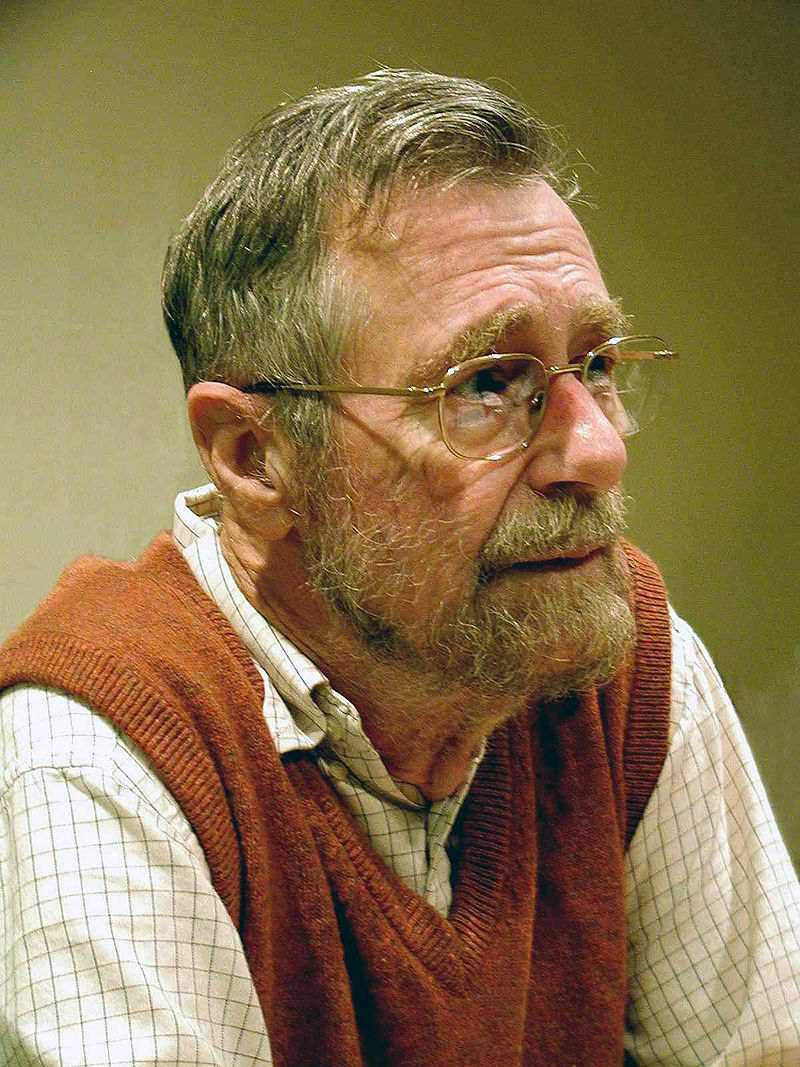
\includegraphics[width=4cm]{images/Edsger_Wybe_Dijkstra}
  \caption{Edgser Wybe Dijkstra (1930-2002)}
  \label{fig:une-autre-image}
\end{figure}

On doit à Dijkstra, qui avait la réputation d'avoir mauvais caractère et de présenter une allergie au ``GOTO'',
quelques citations\footnote{source : \url{https://fr.wikipedia.org/wiki/Edsger_Dijkstra}} telles que :


\begin{quote}
\textit{« Il est pratiquement impossible d'enseigner la bonne programmation aux étudiants 
qui ont eu une exposition antérieure au BASIC : comme programmeurs potentiels, 
ils sont mentalement mutilés, au-delà de tout espoir de régénération. »}
\end{quote}

\begin{quote}
\textit{« Le plus court chemin d'un graphe n'est jamais celui que l'on croit, 
il peut surgir de nulle part, et la plupart du temps, il n'existe pas. »}
\end{quote}

\begin{quote}
\textit{« La programmation par objets est une idée exceptionnellement mauvaise qui ne pouvait naître qu'en Californie. »}
\end{quote}


L'algorithme donne le plus court chemin de la source à \textit{tous les sommets} d'un graphe 
connexe pondéré (orienté ou non) dont le poids lié aux arêtes est positif ou nul.



 %\cite{Roque2012,Roque2012b,Roque2012c,Roque2012d}. 
 


\begin{figure}[htp]
  \centering
  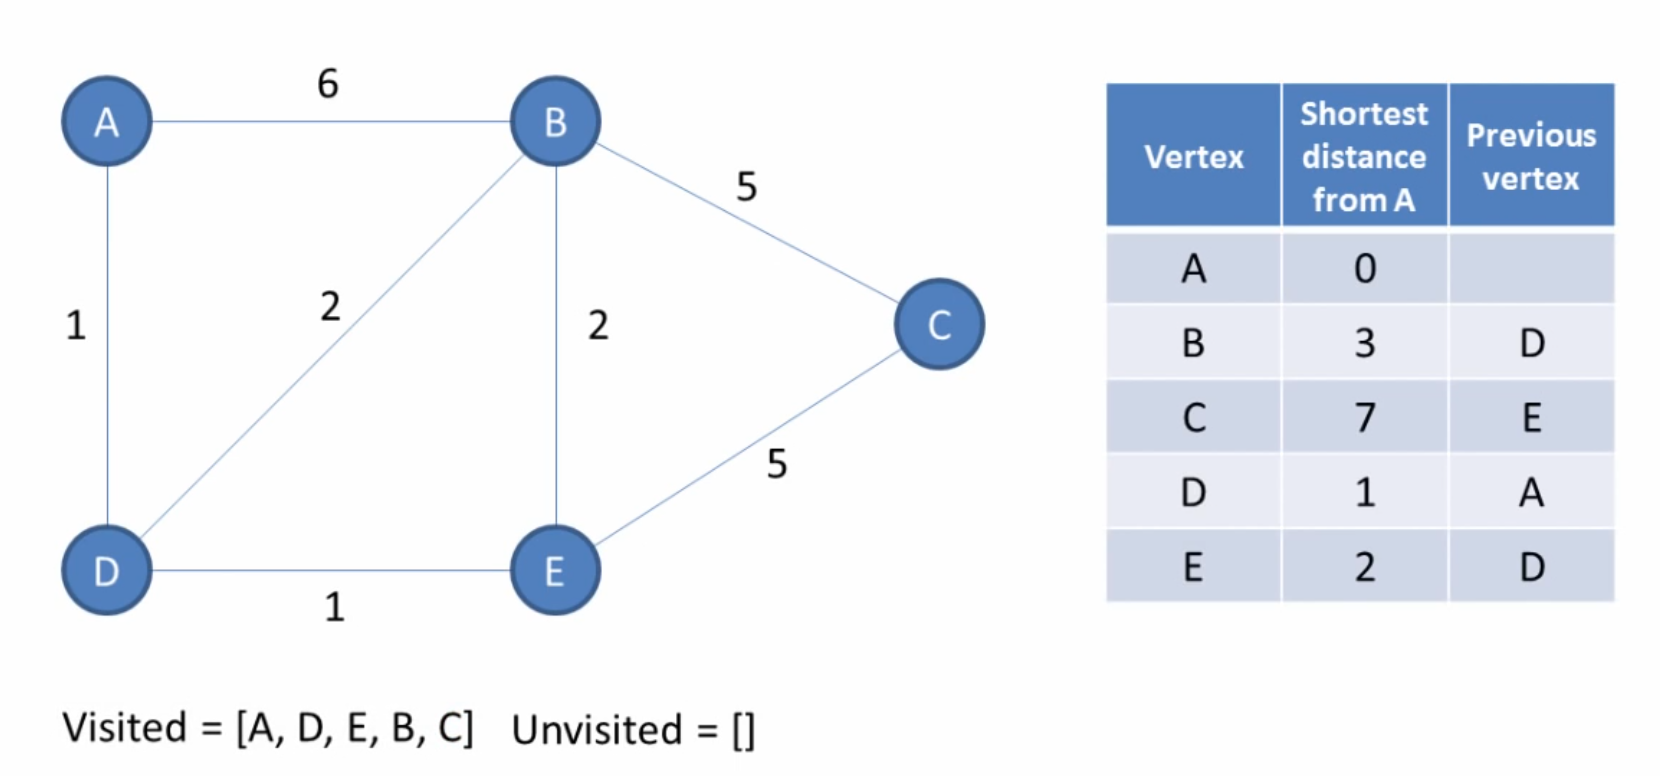
\includegraphics[width=15cm]{images/algo_dij}
  \caption{Exemple de calcul des plus courts chemins à partir du noeud A.}
  \label{fig:une-autre-image}
\end{figure}

L'algorithme de Disjkstra est un algorithme glouton qui utilise l'hypothèse qu'une décision prise sur la base
d'un critère d'optimalité locale conduira à un optimum global. Ainsi, à chaque itération, l'algorithme choisit le noeud
du réseau dont la distance au noeud de départ est la plus faible.
% \begin{figure}[htp]
%   \centering
%   \tikzstyle{block} = [draw, fill=blue!20, rectangle, minimum height=3em, minimum width=6em, text width=6em,text centered]
\begin{tikzpicture}[auto, node distance=3.5cm,>=latex']
\shorthandoff{:} % Evite le bug de compilation avec tikz
    % Longueurs et espacement
    \def\longabove{0.2cm}
    \def\espacement{4cm}

    % Définition des blocs
    \node [block, node distance=\espacement] (codeur) {Codeur};
    \node [block, right of=codeur, node distance=\espacement] (cbs) {CBS};
    \node [block, right of=cbs, node distance=\espacement] (modulateur) {Modulateur};
 
    % Définition des liens
    \draw [<-] (codeur) -- ++(-2,0) node[left] {$\{b_n\}$};
    \draw [->] (codeur) -- node[above=\longabove] {$\{d_n\}$} (cbs);
    \draw [->] (cbs) -- node[above=\longabove] {$\{c_k\}$} (modulateur);
    \draw [->] (modulateur) -- ++(2,0) node[right] {$s(t)$};
\end{tikzpicture}

%   \caption{Exemple de diagramme TikZ.}
%   \label{fig:une-image}
% \end{figure}

\section{Algorithme A*}
Lorem ipsum dolor sit amet, consectetur adipiscing elit. Sed non risus. Suspendisse l
\section{Utilisation}

Dijkstra est utilisé dans le routaghe dynamique OSPF
Comment les utiliser pour transférer de façon optimale une donnée d'un noeud à un autre. 

\begin{table}[ht]
  \begin{center}
    \begin{tabular}{|c|c|c|c|c|}
      \hline
      & $h(t,\tau)$ & $S_{\OP{H}}^{(\alpha)} (f,\tau)$ & $L_{\OP{H}}^{(\alpha)} (\nu,t)$ & $H^{(\alpha)}(f,\nu)$ \\
      \hline
      LTI & $q(\tau)$ & $q(\tau) \delta(f)$ & $Q(\nu)$ & $Q(\nu) \delta(\nu-f)$ \\
      \hline
      LFI & $m(t) \delta(\tau)$ & $M(f) \delta(\tau)$ & $m(t)$ & $M(f)$\\
      \hline
      identité & $\delta(t)$ & $\delta(f)\delta(\tau)$ & $1$ & $\delta(\nu-f)$\\
      \hline
    \end{tabular}
    \caption{Exemple de tableau.}
    \label{tab:un-tableau}
  \end{center}
\end{table}

Lorem ipsum dolor sit amet, consectetur adipiscing elit. Sed non risus. Suspendisse lectus tortor, dignissim sit amet, adipiscing nec, ultricies sed, dolor. Cras elementum ultrices diam. Maecenas ligula massa, varius a, semper congue, euismod non, mi. Proin porttitor, orci nec nonummy molestie, enim est eleifend mi, non fermentum diam nisl sit amet erat. Duis semper. Duis arcu massa, scelerisque vitae, consequat in, pretium a, enim. Pellentesque congue. Ut in risus volutpat libero pharetra tempor. Cras vestibulum bibendum augue. Praesent egestas leo in pede. Praesent blandit odio eu enim. Pellentesque sed dui ut augue blandit sodales. Vestibulum ante ipsum primis in faucibus orci luctus et ultrices posuere cubilia Curae; Aliquam nibh. Mauris ac mauris sed pede pellentesque fermentum. Maecenas adipiscing ante non diam sodales hendrerit. Ut velit mauris, egestas sed, gravida nec, ornare ut, mi. Aenean ut orci vel massa suscipit pulvinar. Nulla sollicitudin. Fusce varius, ligula non tempus aliquam, nunc turpis ullamcorper nibh, in tempus sapien eros vitae ligula. Pellentesque rhoncus nunc et augue. Integer id felis. Curabitur aliquet pellentesque diam. Integer quis metus vitae elit lobortis egestas. Lorem ipsum dolor sit amet, consectetuer adipiscing elit. Morbi vel erat non mauris convallis vehicula. Nulla et sapien. Integer tortor tellus, aliquam faucibus, convallis id, congue eu, quam. Mauris ullamcorper felis vitae erat. Proin feugiat, augue non elementum posuere, metus purus iaculis lectus, et tristique ligula justo vitae magna. Aliquam convallis sollicitudin purus. Praesent aliquam, enim at fermentum mollis, ligula massa adipiscing nisl, ac euismod nibh nisl eu lectus. Fusce vulputate sem at sapien. Vivamus leo. Aliquam euismod libero eu enim. Nulla nec felis sed leo placerat imperdiet. Aenean suscipit nulla in justo. Suspendisse cursus rutrum augue. Nulla tincidunt tincidunt mi. Curabitur iaculis, lorem vel rhoncus faucibus, felis magna fermentum augue, et ultricies lacus lorem varius purus. Curabitur eu amet (fig. \ref{fig:une-autre-image}).

\begin{figure}[htp]
  \centering
  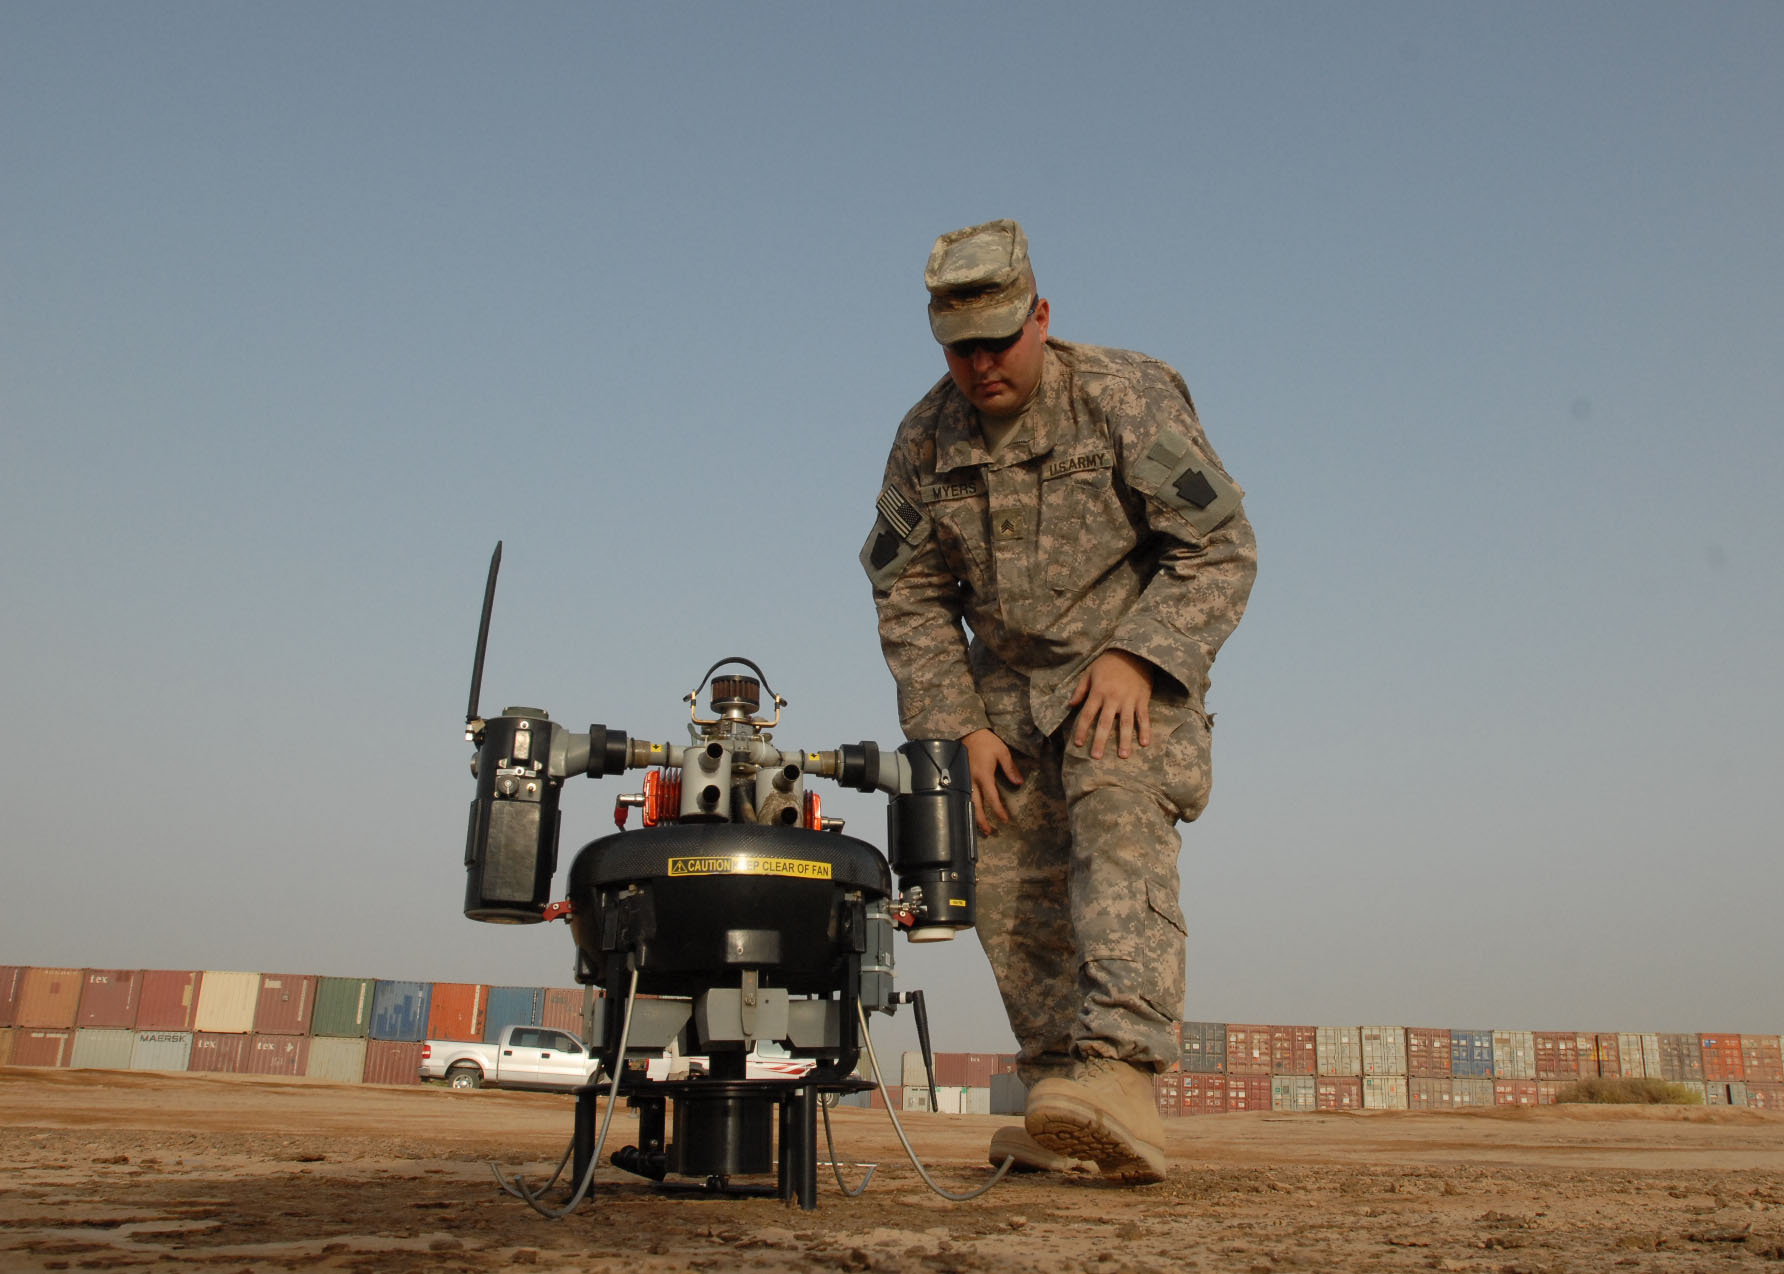
\includegraphics[width=4cm]{images/bitmap_image}
  \caption{Exemple d'image au format JPG.}
  \label{fig:une-autre-image}
\end{figure}


%%% Local Variables: 
%%% mode: latex
%%% TeX-master: "isae-report-template"
%%% End: 